As mentioned in Section \ref{sec:background}, Mondshein himself gave an $O(m^2)$ algorithm to compute his sequence \cite{mond}, later Cheriyan gave an $O(mn)$ time algorithm \cite{cheriyan}.
The main focus of these notes is the linear time algorithm proposed by Schmidt \cite{Schmidt13a} to compute a Mondshein sequence.
At the core of Schimdt's algorithm lies a classical construction of 3-connected graphs proposed by Barnette and Grunbaum \cite{bg} and Tutte [\cite{tutteConnectivity}, Thms. 12.64 and 12.65].
Before describing the Schimidt's algorithm, we will first see what are \textit{BG-Operations}.

\subsection{BG-Operations}

\begin{defn} \label{def:bg}
The following operations on simple graphs are BG-operations (See Fig \ref{fig:bg}):
\begin{enumerate}
\item \textit{vertex-vertex-addition}: Add an edge between two distinct non-adjacent vertices.
\item \textit{edge-vertex-addition}: Subdivide an edge $ab$, $a \ne b$, by a vertex $v$ and add an edge $vw$ where $w \notin \{a,b\}$.
\item \textit{edge-edge-addition}: Subdivide two distinct edges by vertices $v$ and $w$, respectively, and add the edge $vw$.
\end{enumerate}
\end{defn}

\begin{figure}
    \centering
    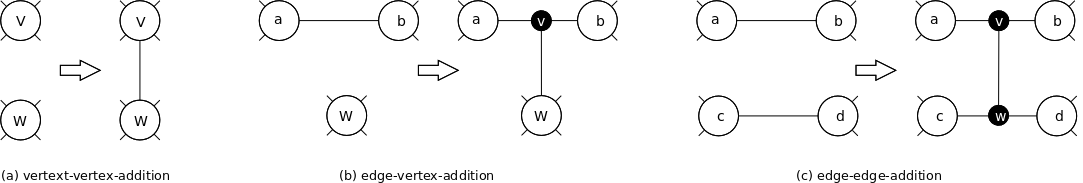
\includegraphics[scale=0.3]{bg.png} \\
    \caption{BG Operations as described in Def. \ref{def:bg}.}
    \label{fig:bg}
\end{figure}

Barnette and Grunbaum, and Tutte also gave the following Theorem:

\begin{thm} \label{thm:k4bg}
(\cite{bg}, \cite{tutteConnectivity}). A graph is 3-connected if and only if it can be constructed from $K_4$ using the \textit{BG-operations}.
\end{thm}

It can be seen from Theorem \ref{thm:k4bg} that applying BG-operation on 3-connected graphs keeps them simple and 3-connected.
Figure \ref{fig:bgEg} gives an example of obtaining $K_5$ from $K_4$ using BG-operations.
A sequence of BG-operations that construct G from $K_4$ is known as \textit{BG-sequence}.
Theorem 6 and 52 in \cite{bgLinear} shows that BG-sequence of a 3-connected graph can be computed in time $O(m)$.
\begin{figure}
    \centering 
    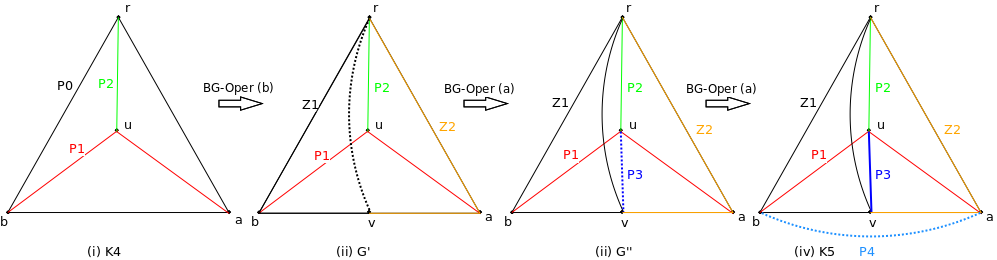
\includegraphics[scale=0.27]{bgEg.png} \\ 
    \caption{Obtaining $K_5$ from $K_4$ using BG-operations. Pi and Zi shows the ear decomposition. Dotted line denotes the newly added edge.}
    \label{fig:bgEg}
\end{figure}



\subsection{Algorithm}
We will first give an overview of the algorithm and later go into the detailed cases.
The algorithm starts with computing a Mondshein sequence of $K_4$, which is easy.
Then using Theorem \ref{thm:k4bg} we construct our G in a step by step manner from $K_4$, this can be done in linear time, as BG-sequence can be computed in linear time.
Our claim is that, each BG-operation in the BG-sequence of $G'$ to G, modifies the Mondshein sequence in a well defined way given by Lemma \ref{lem:cases}.
In other words there are finite number of cases to which each BG-operation can be mapped while transforming G' to G, and each of those cases have finite number of additions to the Mondshein sequence of G'.
This gives us a Mondshein sequence of G from the Mondshein sequence of G'.

\begin{exmp}
For example, Figure \ref{fig:bgEg} explains the changes in Mondshein sequence when obtaining $K_5$ from $K_4$.
Mondshein sequence of $K_4$ is [P0, P1, P2] (follow the color coding).
After applying $BG-Oper(b)$ on $K_4$, which maps to case 2aiii of Lemma \ref{lem:cases} (defined later), we get G' and mondshein sequence is [Z1, Z2, P1, P2].
After $BG-Oper(a)$ on G', which maps to case 1 of Lemma \ref{lem:cases}, we get G'' and Mondshein sequence is [Z1, Z2, P1, P2, P3].
In the final operation $BG-Oper(a)$ which again maps to case 1 of Lemma \ref{lem:cases}, we get $K_5$ and final Mondshein sequence is [Z1, Z2, P1, P2, P3, P4].
\end{exmp}

Now we will define some notations for describing the modifications.
Let $\Gamma$ be a single BG-operation, that adds edge $vw$, if applicable, as described in Def. \ref{def:bg}.
Whenever we consider edges $ab$ and $cd$, without loss of generality (w.l.o.g) we assume that $birth(a) \leq birth(b), birth(c) \leq birth(d)$ and $birth(d) \leq birth(b)$.
Let set $S \subseteq \{av,vb,vw,cw,wd\}$ be the set of new edges added after operation $\Gamma$, see figure \ref{fig:bg}.

The following Lemma describes a detailed scheme of modifying Mondshein sequence for each possible scenario of applying $\Gamma$ on G.

\begin{lem} \label{lem:cases}
There is a Mondshein sequence $D' = (P_0',P_1',...,P_{k+1}')$ of G' avoiding ru (respectively, rv or rw if applicable) that can be obtained from $D = (P_0,P_1,...,P_k)$ of G by performing the following four modifications:

\begin{enumerate}
\item[M1)] replacing the long ear $P_{birth(b)}$ with $P_{b1}', P_{b2}', P_{b3}'$ in order and if applicable. Each $P_{bi}'$ consists of edges in $P_{birth(b)} \cup S$.
\item[M2)] if $P_{birth(cd)}$ is a long ear and $birth(d) < birth(b)$, subdivide $cd$ with $w$ and replace $P_{birth(cd)}$ with the long ear $P_{birth(cwd)}'$.
\item[M3)] if $P_{birth(ab)}$ is short, delete or replace $P_{birth(ab)}$ with an edge in \{av,vb,vw\}; if $P_{birth(cd)}$ is short, delete or replace $P_{birth(cd)}$ with an edge in \{cw,wd\}.
\item[M4)] adding vw as new last ear, if applicable.
\end{enumerate}

In particular, each $\Gamma$ lies in one of the following cases and defines the construction of D' from D, also shown in Fig. \ref{fig:algoCases} :
\begin{enumerate}
\item $\Gamma$ is a vertex-vertex-addition: use M4.
\item $\Gamma$ is an edge-vertex-addition: This case will depend whether b is an inner vertex or not
	\begin{enumerate}
	\item w.l.o.g. birth(b) = birth(ab), i.e. b is an inner-vertex.
	Let a' and b' be the endpoints of $P_{birth(b)}$ such that a' is closer to a than to b.
	Let $P_{avb}'$ be the path obtained by subdividing ab in $P_{birth(b)}$ with v.
	This will have three cases depending upon w's position:
		\begin{enumerate}
		\item $w \notin G_{birth(b)}$ i.e. $birth(w) > birth(b)$ \\
		Obtain $P_{avb}'$ from $P_{birth(b)}$ and add ear vw at the end.
		\item $w \in G_{birth(b)} - P_{birth(b)}$ i.e. $birth(w) < birth(b)$ and $w \notin \{a',b'\}$ \\
		Obtain $P_{avb}'$ from $P_{birth(b)}$ and replace $P_{birth(b)}$ with $Z_1 = a'w-path$ and $Z_2 = vb'-path$ in this order to obtain D'.
		\item $w \in P_{birth(b)}$ i.e. $birth(w) = birth(b)$ or $w \in \{a',b'\}$ \\
		Obtain $Z = P_{avb}'$ from $P_{birth(b)}$. Let $Z_2 = vw-path$, $Z_1 = Z - Z_2 + vw$.
		(If $P_{birth(b)}$ is $P_0$ then there will be two vw-path, choose the one not containing r as an inner vertex.)
		Get D' by replacing $P_{birth(b)}$ with $Z_1$ and $Z_2$ in this order, (from now on we will call this process as applying $M1(Z_1,Z_2,\o)$, with $P_{b1}'=Z_1, P_{b2}'=Z_2, P_{b3}' = \o $.)
		\end{enumerate}
	\item w.l.o.g. birth(b) $<$ birth(ab) and $P_{birth(ab)} = ab$, i.e. b is not an inner vertex. Note that ear $P_{birth(ab)}$ cannot be long as a and b have to be born before ab.
	Again three cases depending upon w's position:
		\begin{enumerate}
		\item $birth(w) > birth(b)$ \\
		Replace $P_{birth(ab)} = ab$ with ear $av \cup vb$ and add ear ear vw at the end.
		\item $birth(w) < birth(b)$: cases depending upon a's relation with b.
			\begin{enumerate}
			\item $birth(a) < birth(b)$ \\
			If ab = ru, add new ear $wv \cup vu$ directly after $P_{birth(u)}$ and replace $P_{birth(ru)} = ru$ with rv.
			If ab $\neq$ ru, add new ear $av \cup vw$ directly after $P_{birth(b)-1}$ and replace $P_{birth(ab)} = ab$ with vb.
			\item $birth(a) = birth(b)$ \\
			Let $Z_1 = av \cup vw \cup P_{birth(b)}[a',a]$ and $Z_2 = P_{birth(b)}[a,b']$. Apply $M1(Z_1,Z_2,\o)$ and replace $P_{birth(ab)} = ab$ with vb.
			\end{enumerate}
		\item $birth(w) = birth(b)$ \\
		If $birth(a) = birth(b) > 0$, let a' and b' be the endpoints of $P_{birth(b)}$ such that a' is closer to a than to b.
		Cases depending upon a's relation with b:
			\begin{enumerate}
			\item $birth(a) = birth(b) > 0$ and w lies strictly between either a and a' or b and b' in $P_{birth(b)}$, (say w.l.o.g. between b and b') \\
			Let $Z_1 = av \cup vw \cup P_{birth(b)}[a',a] \cup P_{birth(b)}[w,b'] $ and $Z_2 = P_{birth(b)}[a,w]$.
			Apply $M1(Z_1,Z_2,\o)$ and replace $P_{birth(ab)} = ab$ with vb.
			\item $birth(a) = birth(b) > 0$ and w lies strictly between a and b in $P_{birth(b)}$.\\
			Let $Z_1 = av \cup vb \cup P_{birth(b)}[a',a] \cup P_{birth(b)}[b,b'] $ and $Z_2 = P_{birth(b)}[a,b]$.
			Apply $M1(Z_1,Z_2,\o)$ and replace $P_{birth(ab)} = ab$ with vw.
			\item $birth(a) = birth(b) = 0$ \\
			In this case we are at $P_0$, consider $P_0 = P_{ab} \cup P_{bw} \cup P_{wa}$, one of these path must contain r, say $P_{ab}$.
			Let Z be the union of remaining two paths, $Z = P_{bw} \cup P_{wa}$.
			Let $P_0'$ be the cycle 'arbva', and $Z_2 = Z$ added directly after $P_0'$, and replacing $P_{birth(ab)} = ab$ with vw, i.e. connect v to vertex $j \in \{a,b,w\}$ that is not an endpoint of Z.
			\item $birth(a) < birth(b)$ \\
			Let b' and b'' be the two endpoints of $P_{birth(b)}$ such that b' is closer to w than to b.
			If $b' \neq a$, $Z_1 = av \cup vw \cup P_{birth(b)}[w,b']$ and $Z_2 = P_{birth(b)}[w,b'']$.
			If $b' = a$,  $Z_1 = av \cup vb \cup P_{birth(b)}[b',b'']$ and $Z_2 = P_{birth(b)}[b,b']$.
			Apply $M1(Z_1,Z_2,\o)$ and replace $P_{birth(ab)} = ab$ with vw.
			\end{enumerate}
		\end{enumerate}
	\end{enumerate}
\item $\Gamma$ is an edge-edge-addition: It will again depend whether b is an inner vertex or not. 
(Due to space constraints we will only see 2 of the 13 cases described in \cite{Schmidt13a}.)
	\begin{enumerate}
	\item[3aiA)] $birth(b)=birth(ab)$ (inner vertex), $birth(d) < birth(b)$ and $birth(cd) < birth(b)$.\\
	Let a' and b' be the endpoints of $P_{birth(b)}$ such that a' is closer to a than to b.
	Subdivide ab with v. Then $Z_1 =  P_{birth(b)}[a',v] \cup vw$ and $Z_2 =  P_{birth(b)}[v,b']$.
	$P_{birth(cd)}$ can be short or long. If $P_{birth(cd)} = cd$ (i.e. short), delete $P_{birth(cd)}$ and apply $M1(cw \cup wd, Z_1, Z_2)$.
	If $P_{birth(cd)}$ is long, apply M2 and $M1(Z_1, Z_2, \o)$.
	\item[3biiC)] birth(b) $<$ birth(ab) and $P_{birth(ab)} = ab$, $birth(d) = birth(b)$, $birth(a) < birth(b)$ and $C \notin P_{birth(b)}$. \\
	Then $P_{birth(cd)} = cd$, have to be a short ear, because $C \notin P_{birth(b)}$, $birth(d) = birth(b)$ and $birth(c) < birth(d)$.
	Let b' and b'' be the two endpoints of $P_{birth(b)}$ such that b' is closer to d than to b on $P_{birth(b)}$ (a may be in $\{b',b'',c\}$).
	There can be cases where b=d, and b=d and $ru\in \{ab,cd\}$, but due to space constraint we will not go into their details.
	Consider $b \neq d$, $Z_1 =  P_{birth(b)}[d,b'] \cup cw \cup wd$, $Z_2 = av \cup vw$ and $Z_3 =  P_{birth(b)}[d,b'']$.
	Apply $M1(Z_1,Z_2,Z_3)$, delete $P_{birth(cd)} = cd$ and replace $P_{birth(ab)} = ab$ with vb.
	\end{enumerate}
\end{enumerate}
\end{lem}

\begin{figure}
    \centering
    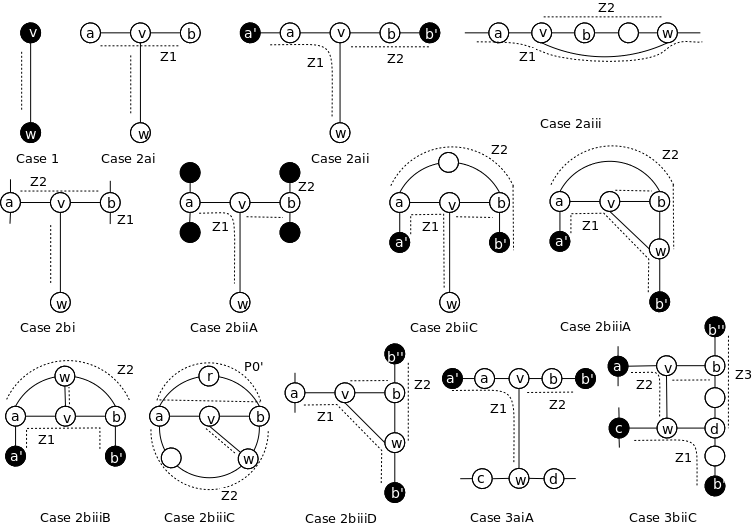
\includegraphics[scale=0.3]{algoCases.png} \\
    \caption{Case 1, 2 and 3 of the Lemma \ref{lem:cases}. Black vertices are the endpoints of the ears that are contained in $G_{birth(b)}$. Dashed paths are part of the ears in D'.}
    \label{fig:algoCases}
\end{figure}

